Consider the polynomials $\phi_1(x) = 1$, $\phi_2(x) = x$, 
and $\phi_3(x) = 3x^2-1$, which form a basis for the set
of all quadratic polynomials.  Use this basis to find the
best quadratic approximation of the form
$f_3(x) = c_1 \phi_1(x) + c_2\phi_2(x) + c_3 \phi_3(x)$
to $f(x) = \cos(\pi x)$ over the interval
$[-1,1]$, given the inner product
\[ \ip{u,v} = \int_{-1}^1 u(x)v(x)\, dx.\]



%%%%%%%%%%%%%%%%%%%%%%%%%%%%%%%%%%%%%%%%%%%%%%%%%%%%%%%%%%%%%%%%%%%%%%%%%%%%%%%%

\ifthenelse{\boolean{showsols}}{\begin{solution}

We can find the coefficients of $f_3(x) = c_1 \phi_1(x) + c_2 \phi_2(x) + c_3 \phi_3(x)$
by solving the linear system:
% \[ \pmatrix{ \ip{\phi_1,\phi_1} & \ip{\phi_1,\phi_2} & \cdots & \ip{\phi_1,\phi_n} \cr
%              \ip{\phi_2,\phi_1} & \ip{\phi_2,\phi_2} & \cdots & \ip{\phi_2,\phi_n} \cr
%                    \ddots       &    \ddots          & \ddots & \vdots  \cr
%              \ip{\phi_n,\phi_1} & \ip{\phi_n,\phi_2} & \cdots & \ip{\phi_n,\phi_n}}
%    \pmatrix{c_1 \cr c_2 \cr \vdots \cr c_n}
%   = \pmatrix{ \ip{\phi_1, f} \cr 
%               \ip{\phi_2, f} \cr
%                \vdots \cr
%               \ip{\phi_n, f}} \]
\[ \pmatrix{ \ip{\phi_1,\phi_1} & \ip{\phi_1,\phi_2} & \ip{\phi_1,\phi_3} \cr
             \ip{\phi_2,\phi_1} & \ip{\phi_2,\phi_2} & \ip{\phi_2,\phi_3} \cr
             \ip{\phi_3,\phi_1} & \ip{\phi_3,\phi_2} & \ip{\phi_3,\phi_3}}
   \pmatrix{c_1 \cr c_2 \cr c_3}
  = \pmatrix{ \ip{\phi_1, f} \cr 
              \ip{\phi_2, f} \cr
              \ip{\phi_3, f}} \]
First we must determine the coefficients of the matrix, which is the simple
matter of integrating polynomials:
\begin{eqnarray*}
  \ip{\phi_1,\phi_1} &=& \int_{-1}^1 1^2\,dx = 2 \\[0.5em]
  \ip{\phi_2,\phi_1} = \ip{\phi_1, \phi_2} 
                     &=& \int_{-1}^1 1\cdot x\,dx = 0 \\[0.5em]
  \ip{\phi_3,\phi_1} = \ip{\phi_1, \phi_3} 
                     &=& \int_{-1}^1 1 (3x^2-1)\,dx = 0 \\[0.5em]
  \ip{\phi_2,\phi_2} &=& \int_{-1}^1 x^2\,dx = 2/3 \\[0.5em]
  \ip{\phi_3,\phi_2} = \ip{\phi_3, \phi_2} 
                     &=& \int_{-1}^1  x (3x^2-1)\,dx = 0 \\[0.5em]
  \ip{\phi_3,\phi_3} &=& \int_{-1}^1 (3x^2-1)^2\,dx = 8/5,
\end{eqnarray*}
hence the basis vectors are orthogonal.
The entries of the vector on the right-hand side can be computed 
using integration by parts:
\begin{eqnarray*}
  \ip{\phi_1,f} &=& \int_{-1}^1 1\cdot\cos(\pi x)\,dx = 0 \\[0.5em]
  \ip{\phi_2,f} &=& \int_{-1}^1 x\cdot\cos(\pi x)\,dx = 0 \\[0.5em]
  \ip{\phi_3,f} &=& \int_{-1}^1 (3x^2-1)\cdot\cos(\pi x)\,dx = -12/\pi^2.\\[0.5em]
\end{eqnarray*}
Since the matrix is diagonal, the coefficients $c_1$, $c_2$, and $c_3$ are simple to find:
\begin{eqnarray*}
    c_1 &=& \ip{\phi_1,f}/\ip{\phi_1,\phi_1} = 0 \\[0.5em]
    c_2 &=& \ip{\phi_2,f}/\ip{\phi_2,\phi_2} = 0 \\[0.5em]
    c_3 &=& \ip{\phi_3,f}/\ip{\phi_3,\phi_3} = -15/(2\pi^2).
\end{eqnarray*}
Thus the best approximation to $\cos(\pi x)$ from the quadratic polynomials is
\[ f_3(x) = {15\over 2\pi^2} (1-3x^2).\]

We plot compare the best approximation to $f(x)$ in the following plot
(not requested in this problem).  As one would expect, the approximation 
diverges from $f(x)$ outside the interval $[-1,1]$.

\begin{equation} 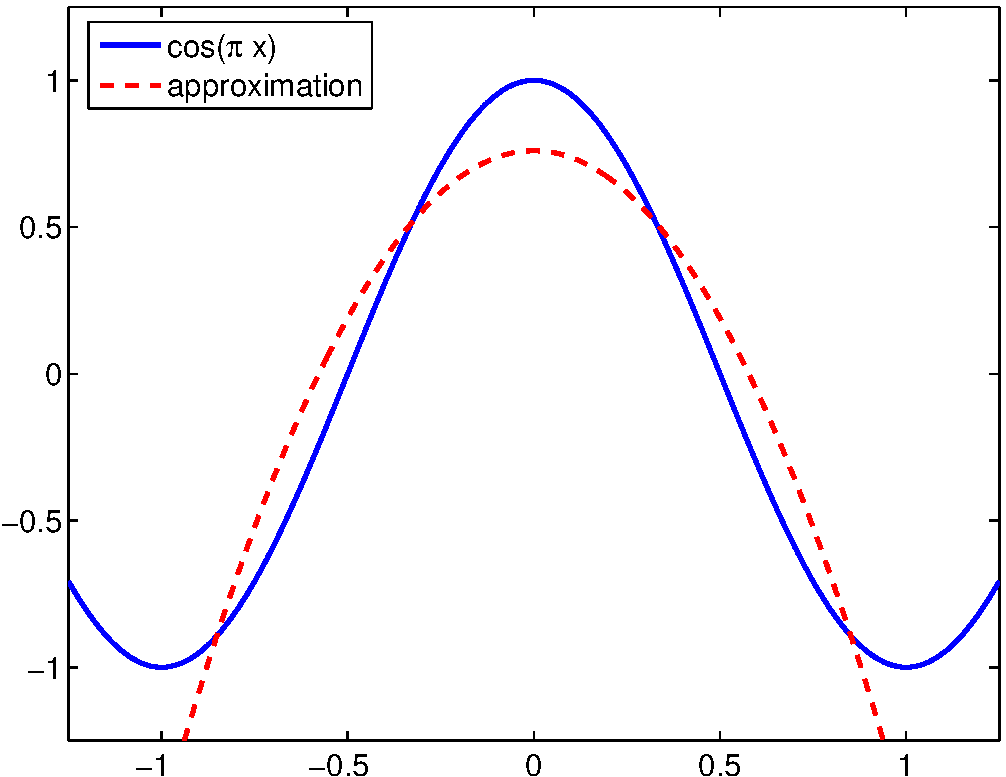
\includegraphics[scale=0.5]{legendre} \end{equation}

\end{solution}}{}

